\section{Технический проект}
\subsection{Общая характеристика организации решения задачи}

Необходимо спроектировать и разработать приложение, который должен способствовать популяризации платформер игр.

Приложение представляет собой набор взаимосвязанных различных окон, которые сгруппированы по разделам, содержащие текстовую, графическую информацию. Приложение располагается на компьютере.

\subsection{Обоснование выбора технологии проектирования}

На сегодняшний день информационный рынок, поставляющий программные решения в выбранной сфере, предлагает множество продуктов, позволяющих достигнуть поставленной цели – разработки игрового приложения.

\subsubsection{Описание используемых технологий и языков программирования}

В процессе разработки приложения используются программные средства и языки программирования. Каждое программное средство и каждый язык программирования применяется для круга задач, при решении которых они необходимы.

\subsubsection{Язык программирования Python}

Python –  высокоуровневый язык программирования общего назначения с динамической строгой типизацией и автоматическим управлением памятью, ориентированный на повышение производительности разработчика, читаемости кода и его качества, а также на обеспечение переносимости написанных на нём программ. Язык является полностью объектно-ориентированным в том плане, что всё является объектами. Необычной особенностью языка является выделение блоков кода отступами. Синтаксис ядра языка минималистичен, за счёт чего на практике редко возникает необходимость обращаться к документации. Сам же язык известен как интерпретируемый и используется в том числе для написания скриптов. Недостатками языка являются зачастую более низкая скорость работы и более высокое потребление памяти написанных на нём программ по сравнению с аналогичным кодом, написанным на компилируемых языках, таких как C или C++.

\subsubsection{Язык программирования Python}

\paragraph{Достоинства языка Python}
\begin{itemize}
	\item Простота и читаемость кода: Python использует простой и чистый синтаксис, что делает код легким для понимания и обслуживания.
	\item Многофункциональность: Python подходит для создания различных типов приложений, включая веб-приложения, настольные приложения, научные вычисления, обработку данных и многое другое
	\item Большой выбор библиотек: Python имеет огромное сообщество разработчиков, что приводит к большому количеству библиотек и модулей для различных задач. Например, для машинного обучения есть библиотека TensorFlow, для веб-разработки - Django, для анализа данных - Pandas и многое другое.
	\item Кроссплатформенность: Python работает на различных операционных системах, таких как Windows, macOS, Linux и другие.
	\item Быстрая разработка: Python позволяет быстро создавать прототипы и тестировать идеи благодаря своей простоте и мощности.
\end{itemize}

\paragraph{Недостатки языка Javascript}

\begin{itemize}
	\item Низкая производительность: Python может быть медленнее других языков программирования, таких как C++ или Java, особенно при выполнении вычислительно сложных операций.
	\item Глобальная блокировка интерпретатора: из-за глобальной блокировки GIL (Global Interpreter Lock) в Python, многопоточные приложения могут испытывать проблемы с параллельным выполнением кода.
	\item Не самый подходящий для мобильной разработки: Python не является первым выбором для мобильной разработки из-за ограниченной поддержки на мобильных платформах.
	\item Не все библиотеки могут быть на Python: Так как Python находится в постоянном развитии, не все библиотеки могут быть доступны на этом языке.
	\item Меньшая поддержка для некоторых областей разработки, таких как игровая разработка или высокопроизводительные вычисления.
\end{itemize}

\subsubsection{Использование библиотеки Tkinter}

\paragraph{Введение}
Библиотека Tkinter - это стандартная библиотека Python для создания графического пользовательского интерфейса (GUI). Она обладает широкими возможностями для создания разнообразных приложений с использованием различных виджетов, таких как кнопки, поля ввода, метки и многое другое.

\paragraph{Возможности Tkinter}
Вот некоторые из основных возможностей, предоставляемых библиотекой Tkinter:

\begin{itemize}
	\item Создание различных виджетов: кнопки, метки, поля ввода, списки и многое другое.
	\item Управление компоновкой виджетов с использованием менеджеров компоновки (например, grid, pack, place).
	\item Обработка событий, таких как щелчок мыши, нажатие клавиш и другие.
	\item Возможность создания различных диалоговых окон, таких как окна предупреждений, информационные окна и окна запроса.
	\item Поддержка многопоточности для обновления интерфейса из различных потоков выполнения.
\end{itemize}

\paragraph{Заключение}
Библиотека Tkinter предоставляет мощные инструменты для создания графических пользовательских интерфейсов на языке Python. Реализация таймеров на Python может быть достигнута с помощью модулей \texttt{time} или \texttt{threading}, в зависимости от конкретных требований приложения.

\paragraph{Описание движка}
PlatformGame - главный класс движка. Создается класс-наследник PsGame. Здесь будут храниться глобальные переменные конкретной игры (например флаги каких-то событий или уровней). Все функции движка там: добавить уровень, перейти на уровень, поместить персонажа/предмет, установить главного персонажа, удалить персонажа, предмет, запустить/остановить сценарий, передать управление в другой сценарий, активировать предмет.
То есть это все то, что должно быть доступно в любом сценарии. Поэтому, надо делать класс PlatformGame статическим.Саму игру мы задаем в конструкторе это класса как множество уровней. 

Уровни (Levels) представляет собой совокупность объектов, а также хранит свою графику. Каждый объект может иметь свой небольшой управляющий сценарий. Эти сценарии работают параллельно, например, несколько объектов могут двигаться одновременно, или происходит одновременная анимация (волна). Каждый сценарий запускается один раз и далее повторяется в цикле.Уровень имеет отдельные сценарии для входа и выхода (то есть запускается один раз при входе героя в уровень и при выходе).К уровням идет обращение по имени (задается при добавлении уровня в движок).
Сценарий входа в уровень может проверять какие-то игровые ситуации и настраивать уровень перед отображением. Сценарий выхода может останавливать какие-то вещи.
Каждый объект в комнате имеет имя и сценарий по взаимодействию с ним по клику клавиши (например использовать усиление).
Также к Levels относятся Enemies(Враги) и Bonuses(усилители,кольца) отвечающие за врагов и лут на уровне.

Персонаж (Tommy) имеют свою анимацию движения по уровню. По клику мыши в точку X,Y (или по программно заданным координатам) происходит автоматическое движение.
В уровни также задаются области (как множество прямоугольников(тайлов)), где происходит движение персонажей.
Tommy может иметь набор предметов или инвентарь.

Graphics отвечает за отрисовку уровня, передвижение "камеры" следующей за персонажем, врагов, предметов.

Анимацию задаем как последовательность кадров с заданной скоростью.
Автоматическое движение объекта задаем в сценарии.

Сценарий запускается (StartScript), и затем работает до тех пор пока не будет остановлен (StopScript).
В сценарии задаем шаги движения, между которыми вызываем Yield (передать управление другому потоку). То есть сценарии - это параллельные потоки.
Глобальные переменные могут быть в классе конкретной игры или в статическом классе Globals. Чтобы к ним обратиться, функция сценария должна также быть в классе игры. Локальные переменные могут быть внутри конкретной комнаты, тогда локальные сценарии находятся в классе комнаты.

Сценарий - это любой метод (например у PsGame или у конкретной комнаты (класса, потомка от Levels).
То есть мы в движок передаем метод (через делегат), а уже сам движок делает все что нужно (запускает поток).
У наследника указываются только свои поля. Сценарии размещаются в зависимости от того, что там делается.
Если просто перемещение, смена состояния, смена уровня - тогда в классе конкретного уровня (потомка Levels).

\subsection{Диаграмма компонентов и схема обмена данными между файлами компонента}

Диаграмма компонентов описывает особенности физического представления разрабатываемой системы. Она позволяет определить архитектуру системы, установив зависимости между программными компонентами, в роли которых может выступать как исходный, так и исполняемый код. Основными графическими элементами диаграммы компонентов являются компоненты, интерфейсы, а также зависимости между ними. На рисунке \ref{comp:image} изображена диаграмма компонентов для проектируемой системы. Она включает в себя сервер с операционной системой, на которой установлена система управления содержимым, включающая в себя базу данных и интерфейс. Помимо этого на диаграмме изображен клиентский компьютер с операционной системой, на которой установлен браузер.

Диаграмма классов платформерного движка представлена на рисунке ~\ref{DimClasses:image}.
\begin{figure}[ht]
	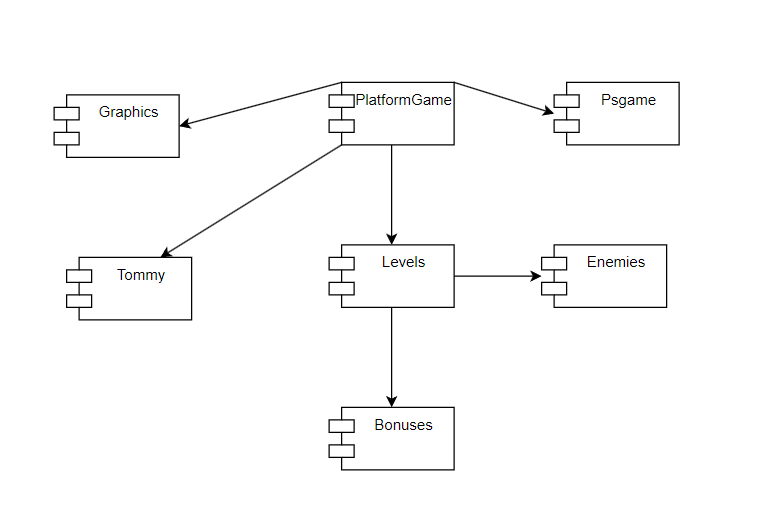
\includegraphics[width=1\linewidth]{DimClasses}
	\caption{Диаграмма классов}
	\label{DimClasses:image}
\end{figure}

 
